\subsection{Simulated populations and a controlled experiment}
\label{num-simworld}

Host fluctuations cannot be separated from changes in mean abundance, transmission,
and parasite losses in the available data. A simulated world allows these quantities
to be controlled while host variability and residence in a steady stage are changed
independently. This simulated world is theory, not evidence from nature. We use it
to examine demographic extinction and to assess what a controlled experiment would
need to measure (Online Resource 1, Section~7.8).

% Sources: virtualworld/protocol.md, report.md; verification/replication/validation-rerun.md, pilot-rerun.md.
Validation preceded the pilot. All five of five gates passed, comprising 190 of 190
registered comparisons of small-noise coefficients, mechanism extensions, the exact
gamma-host case, environmental memory, and constant-host demographic persistence.
A second party implemented separate code and repeated all 190 comparisons, with
190 of 190 passing. The full pilot was then independently repeated for 18 of 18
cells, using 400 populations per cell. These checks establish agreement with the
specified models within registered tolerances.

% Sources: virtualworld/pilot.md and its corrections; fix1-report.md; pilot-rerun-fix1.md.
The pilot crossed fixed-mean host forcing with steady mean stays of 1, 5, and
20 steps. Host variability was specified by the log-host standard deviation
($\sigma=0,0.3,0.6$) and lag-one correlation ($\phi=0,0.6$). Each of 18 cells
contained 200 independent populations, followed for 500 steps. The stationary
arithmetic mean was fixed, although individual schedules had different realized
means. The model used two geometric stages, an exposed mean stay of 2 steps,
and independent Poisson offspring at transfers. Initial abundance was 20
at $\ln R_0=0.05$ ($R_0$ is the constant-environment reproduction number),
with no host feedback. At $\phi=0.6$, the corrected noise-by-stay interaction was
$0.435$ (95\% interval $[0.321,0.549]$). This is the noise-associated increase
in extinction at stay one minus that at stay 20. The original pilot is shown
separately (Fig.~\ref{num-1}).

% Sources: verification/vworld-check/vworld-check.md; virtualworld/matched-generations-fix1.md and fix1-report.md.
However, a fixed calendar horizon gives the longer stay fewer generations of
exposure. Subtracting the constant-host controls does not remove this difference.
In the independent audit, matching reference generations reduced the interaction
to $0.22$--$0.30$, with all five of five pointwise intervals above zero.
At $\ln R_0=0.2$, the interaction was $0.49$ at 500 steps, rather than at
matched generations.
A separate corrected matched-generation run gave planning estimates of 51--61
replicate populations per cell for 80\% power, or ca.\ 244 cultures for the
core $2\times2$ comparison. These are model-conditional planning figures.
They concern marginal power at each reference horizon, not joint power
across horizons or achieved power in a biological trial.

% Sources: virtualworld/q4/report.md, including final clarification; verification/q4-check/q4-check.md; a13/report.md.
Observed host trajectories provide a different check. We replayed 120 selected
compilation series and 71 valid \textit{Tribolium} records, normalized to equal
arithmetic means. The invasion-threshold loss $D$ fell with stay in 709 of 764
adjacent comparisons. These counts include shared controls, and replay does not
establish a natural long-run process. The independent departure ledger classified
220 of 271 primary departures as explained by existing results, 51 of 271 as
requiring the hosts-with-zeros extension (A13), and zero of 271 as unresolved.
That extension now has proofs of a raw-host covariance expansion and an outage
bound under their stated conditions, with completed independent review.
The eventual derivative-sign result remains open for general unbounded hosts
with finite fourth moments. Longer stays therefore do not universally lower $D$.

% Source: notes/decisive-experiment-v2.md, especially sections 6--9 and Refereed.
A controlled experiment would compare constant and fluctuating host supply at a
fixed mean, with independently calibrated residence and survival distributions.
Held high and low densities would measure growth responses, fast and slow
switching would distinguish mean-rate changes from dynamic effects, and a period
sweep would examine sensitivity to timing. Random switching should use complete
independent mirrored pairs, with actual exposure recorded. Extinction must be
retained, and replication must include biological variation, observation error,
and uncertainty in calibrated inputs.
The earlier recommendation of one to six replicates was withdrawn after
review because it included measurement error alone. Held-density counts
also require direct infection and disappearance assays to distinguish
delayed transmission from wasted opportunities.

% Sources: notes/decisive-experiment-v2.md section 9 and Refereed; casestudies/leads/leads.md.
Candidate systems include \textit{Paramecium} with \textit{Holospora}, bacteria
with phage, and \textit{Daphnia} with \textit{Ordospora}. None is established as
feasible for this design. The \textit{Tribolium} archive already contains
fixed-mean flour fluctuations, but no parasites and no controlled equality of
beetle abundance \citep{desharnais2023}. No experiment has been run or
system selected. Density manipulation must first be separated from parasite
removal, and encounter rates, development, offspring production, and counting
must be calibrated. For a parasite, the proposed test is whether time in a
steady stage reduces the cost of variable host access once these quantities
are controlled.

\begin{figure}
\centering
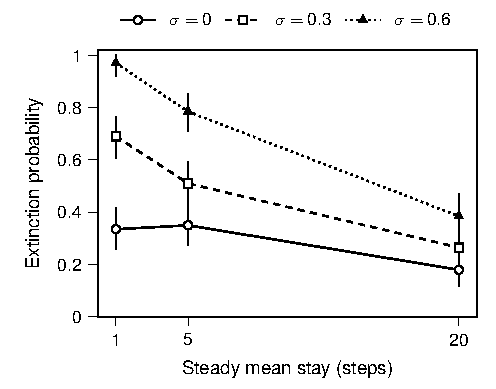
\includegraphics[width=84mm]{figures/num-1.pdf}
\caption{\textbf{Fig. X} Extinction by step 500 in the original pilot at
$\phi=0.6$. Circles with solid lines denote $\sigma=0$, squares with dashed
lines $\sigma=0.3$, and triangles with dotted lines $\sigma=0.6$.
Each point represents 200 independent populations, and bars are pointwise
95\% score intervals. Lines connect the three tested mean stays.
The exposed mean stay is 2 steps, $\ln R_0=0.05$, and initial abundance is 20.
These archived values precede the allocation correction and do not yield the
corrected interaction reported in the text. The horizon is calendar time}
\label{num-1}
\end{figure}
